\section{Annexe}

\begin{figure}[!h]
   \begin{subfigure}[c]{.5\linewidth}
     \centering
     
\includegraphics[scale=0.35]{Chapters/Images/synthetic_map.png}
     \caption{}
   \end{subfigure} 
   \begin{subfigure}[c]{.5\linewidth}
     \centering
     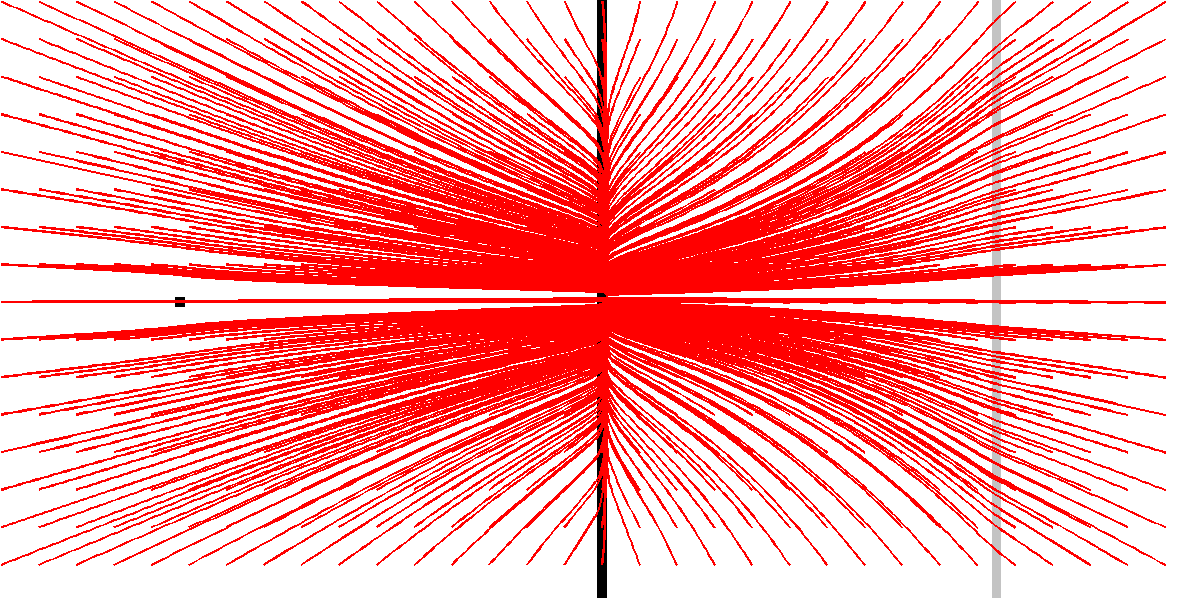
\includegraphics[scale=0.35]{Chapters/Images/m1_gamma_5.png}
     \caption{}
   \end{subfigure} \\
   
   \begin{subfigure}[c]{.5\linewidth}
     \centering
     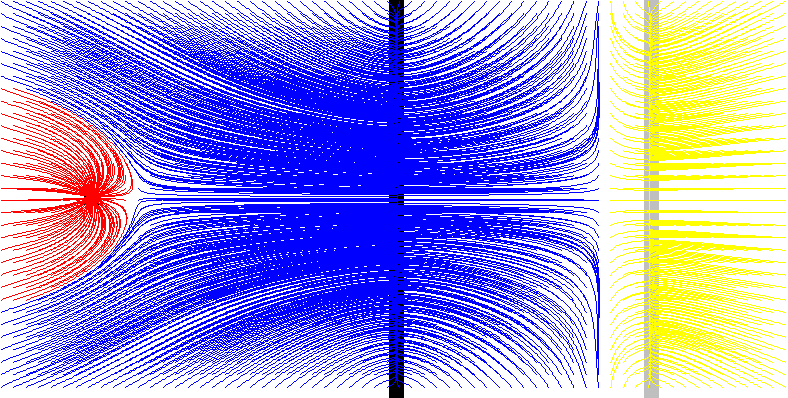
\includegraphics[scale=0.35]{Chapters/Images/synthetic_map_VFC_gamma017.png}
     \caption{}
   \end{subfigure}
   \begin{subfigure}[c]{.5\linewidth}
     \centering
     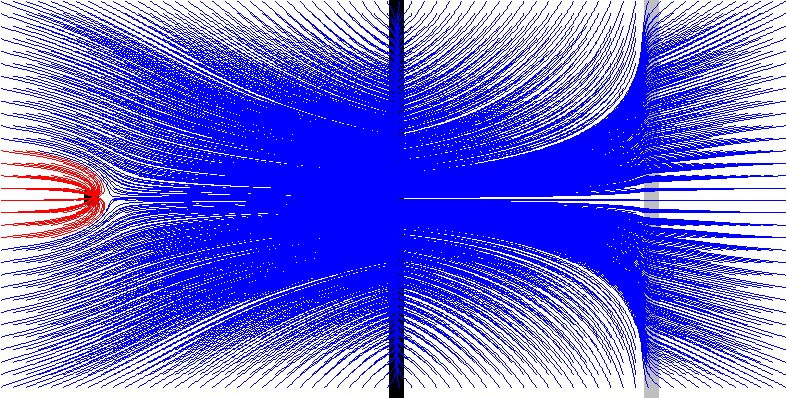
\includegraphics[scale=0.35]{Chapters/Images/synthetic_map_VFC_gamma011.png}
     \caption{}
   \end{subfigure}\\
   
   \caption{(a) Carte de contours $F(x,y)$ synthétique avec un bruit impulsionnel, un contour fort et un contour faible. Lignes de courant générées à partir du champ VFC utilisant $m_1(x,y)$ avec plusieurs valeurs du paramètre $\gamma$ .}
   \label{fig:synthetic_map}
\end{figure}